\documentclass[12pt]{article}
\usepackage[utf8]{inputenc}
\usepackage[T1]{fontenc}
\usepackage[paperwidth=160mm,paperheight=90mm,margin=9mm]{geometry}
\usepackage{xcolor}
\usepackage{graphicx}
\usepackage{hyperref}
\definecolor{forest}{HTML}{183D3B}
\definecolor{paper}{HTML}{F4F1E8}
\definecolor{copper}{HTML}{8A582F}
\pagecolor{paper}\color{forest}
\hypersetup{colorlinks=true,urlcolor=forest,pdftitle={TerraSync: presentación},pdfauthor={404 Gravity Not Found}}
\pagestyle{empty}\setlength{\parindent}{0pt}\setlength{\parskip}{5pt}
\newcounter{slide}
\newcommand{\slide}[2]{\ifnum\value{slide}>0\clearpage\fi\stepcounter{slide}\begingroup{\Large\bfseries #1}\par\vspace{3mm}#2\par\endgroup\vfill{\tiny 404 Gravity Not Found / TerraSync\hfill\arabic{slide}}}
\begin{document}
\slide{TerraSync}{\vspace{6mm}{\Huge El territorio cambia.}\\[3mm]{\Huge Sigue su registro.}\\[6mm]Atlas de observación terrestre de México\\[2mm]\small 404 Gravity Not Found / 15 de noviembre de 2026}
\slide{El problema}{Los registros geoespaciales necesitan contexto.\\[4mm]
\textcolor{copper}{01}\quad ¿Dónde y cuándo ocurrió la señal?\\[3mm]
\textcolor{copper}{02}\quad ¿Qué fuente y evidencia la respaldan?\\[3mm]
\textcolor{copper}{03}\quad ¿Cómo llevo esa selección a mi análisis?}
\slide{Una consulta que conserva su contexto}{\vspace{3mm}{\Large Estado $+$ mes $+$ fenómeno}\\[6mm]
El mismo filtro conecta el mapa, la línea del tiempo, la tabla de Observaciones y el archivo Excel.\\[4mm]
\small Ejemplo: Guerrero, noviembre de 2026; revisar la evidencia y exportar la selección.}
\slide{El catálogo incluido}{\vspace{4mm}
\begin{tabular}{lll}\Huge 3,290 & \Huge 203 & \Huge 32\\[3mm]registros & meses & entidades\end{tabular}\\[7mm]
\small Cifras del artefacto recibido. No implican cobertura uniforme, transmisión en vivo ni validación científica independiente.}
\slide{Explorar sin perder el mapa}{\small
Slider con teclado, arrastre, selector de mes y reproducción.\\[3mm]
Selección de estado con clic o control accesible.\\[3mm]
Controles, lienzo e historial en filas separadas.\\[3mm]
Interfaz ES/EN y tutorial de cuatro pasos.}
\slide{El explorador en funcionamiento}{\centering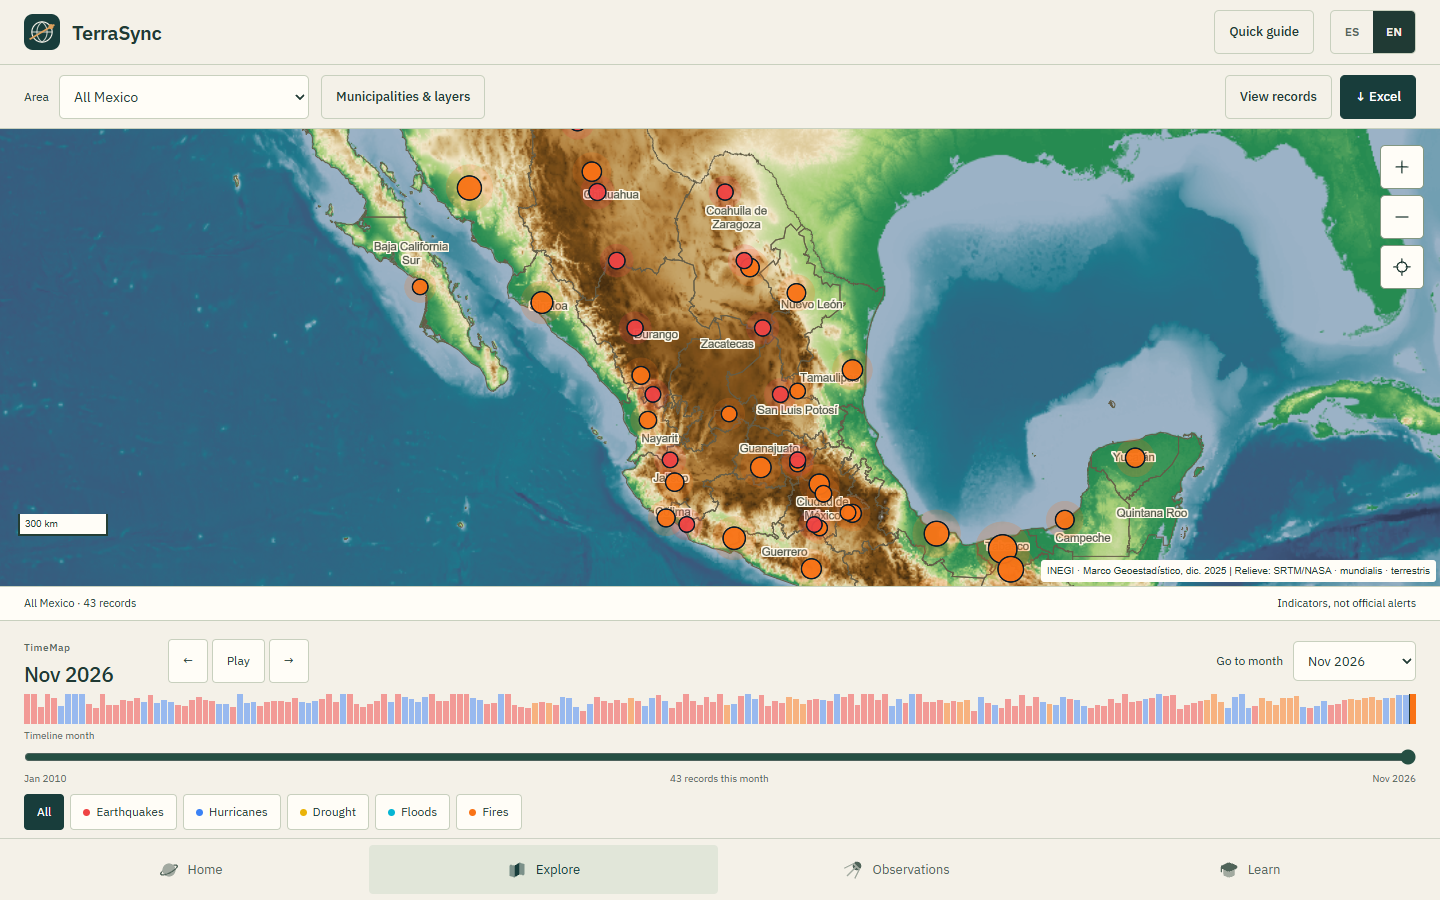
\includegraphics[width=\linewidth,height=51mm,keepaspectratio]{mapa.png}\par}
\slide{Revisar antes de interpretar}{\small
\textbf{observed}: registro marcado como observado.\\[2mm]
\textbf{supervised}: salida etiquetada como supervisada.\\[2mm]
\textbf{proxy}: señal indirecta; requiere contexto.\\[2mm]
\textbf{no\_confirmable}: la evidencia no permite confirmar.\\[4mm]
\footnotesize Una etiqueta no audita la procedencia. Los indicadores no son alertas oficiales.}
\slide{Observaciones y Aprende}{\small
\textbf{Observaciones}\\[2mm]Consulta por mes, estado y fenómeno. Conserva fecha, severidad, evidencia y fuente. Exporta el subconjunto activo.\\[5mm]
\textbf{Aprende}\\[2mm]Introducción al radar, contexto de las señales y lectura de evidencia. Actividad breve y enlaces a NASA.}
\slide{Arquitectura reproducible}{\vspace{2mm}\begin{center}\fbox{React + MapLibre}\quad$\longrightarrow$\quad\fbox{Django REST}\\[4mm]$\downarrow$\\[4mm]\fbox{PostgreSQL + Parquet}\end{center}
\footnotesize Nginx sirve el frontend; Gunicorn ejecuta la API. Credenciales fuera del repositorio.}
\slide{Qué comprobamos}{\small
TypeScript, lint y build del frontend.\\[2mm]
Cinco pruebas de catálogo y exportación, con base temporal.\\[2mm]
Interacciones a 1440, 1024, 768, 390 y 320 px.\\[2mm]
Slider, filtros, idioma, tutorial, tabla y actividad educativa.\\[4mm]
\footnotesize Son pruebas informáticas. No se reportan nuevas métricas científicas.}
\slide{Demostración: del territorio al archivo}{\small
1. Abrir el mapa y seleccionar un estado.\\[2mm]
2. Mover el slider y elegir un fenómeno.\\[2mm]
3. Abrir un punto y revisar su fuente.\\[2mm]
4. Abrir Observaciones y descargar Excel.\\[2mm]
5. Cambiar el idioma y consultar Aprende.}
\slide{Estado de la entrega}{\textbf{Local por decisión del equipo.}\\[4mm]
\small Desarrollo: \texttt{127.0.0.1:5173}\\[2mm]
Perfil Docker: \texttt{127.0.0.1:8080}\\[5mm]
\footnotesize Antes de publicar: dominio y TLS, operación y respaldos, validación independiente del catálogo y nombres de integrantes.}
\slide{TerraSync / 404 Gravity Not Found}{\begin{minipage}[c]{.65\linewidth}{\large Un territorio, una consulta reproducible.}\\[6mm]
\footnotesize\href{https://github.com/GalekTato/404-Gravity-Not-Found}{Ver repositorio en GitHub}\\[5mm]
Nombres personales pendientes de confirmación.\end{minipage}\hfill\begin{minipage}[c]{.3\linewidth}
\includegraphics[width=\linewidth]{../../public/assets/equipo/logo.jpg}\end{minipage}}
\end{document}
